The dynamic project naming script in the code listing for the \texttt{gl}
code example is shown in Figure \ref{fig:naming-code-gl}.  This changes the naming convention of the projects to create
a path containing only the upper-case characters in the namespace path and to use
the project's full name at the end of the abbreviated namespace path.

The example utilizes the SCM's API to get the project details that are not included
with the webhook event payload.\\

\begin{figure}[h]
    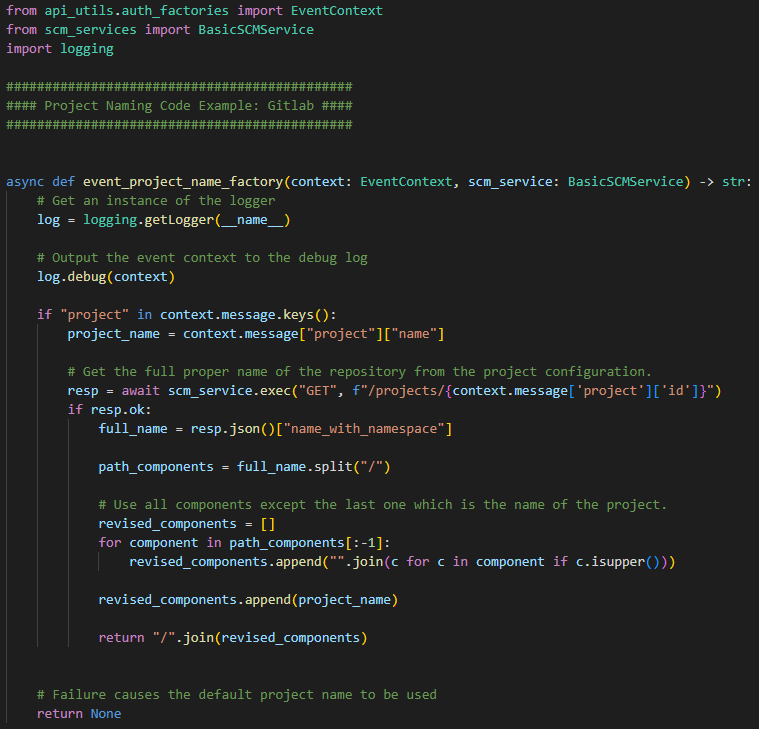
\includegraphics[width=\textwidth]{graphics/naming-code-gl.png}
    \caption{Gitlab Custom Project Naming Code Example}
    \label{fig:naming-code-gl}
\end{figure}
